Current triggering strategy used in the OPQMakai and OPQBox relies on the a triggering stream of three metrics in order to perform anomaly detection. These metrics are THD, fundamental frequency and $V_{rms}$. All three of these metrics are computed over an adjustable temporal window, however since these metrics rely on convolution and averaging, the width of the window influences a minimum width of an anomaly which could be detected. a short transient will be "washed out" in the averaging of the $V_{rms}$ measurement, filtered out in the in the fundamental frequency calculation, and due to the uncertainty principle, have a minimal impact on the THD measurement. I propose to add another metric to the triggering stream, capable of detecting short temporal anomalies regardless of the temporal window size. My method is similar to a highly aggressive lossy wavelet compression, and aims to find frequency disturbances which are not harmonics of the utility frequency. Steps of the proposed wavelet anomaly metric algorithm are shown in figure \ref{expdes:fig:1}. First step involves filtering out the fundamental frequency and its harmonics from the input window. This is accomplished using filtering in frequency domain using FFT. The simplifies further analysis, and removes redundancy, since the mains frequency and its harmonics are already monitored via THD calculation. Next the filtered signal is transformed back into time domain. Finally a discrete wavelet transform is performed on the time domain signal, and the position, level, and magnitude of the highest coefficients are sent as a part of the triggering stream. 

\begin{figure}[h]
	\centering
	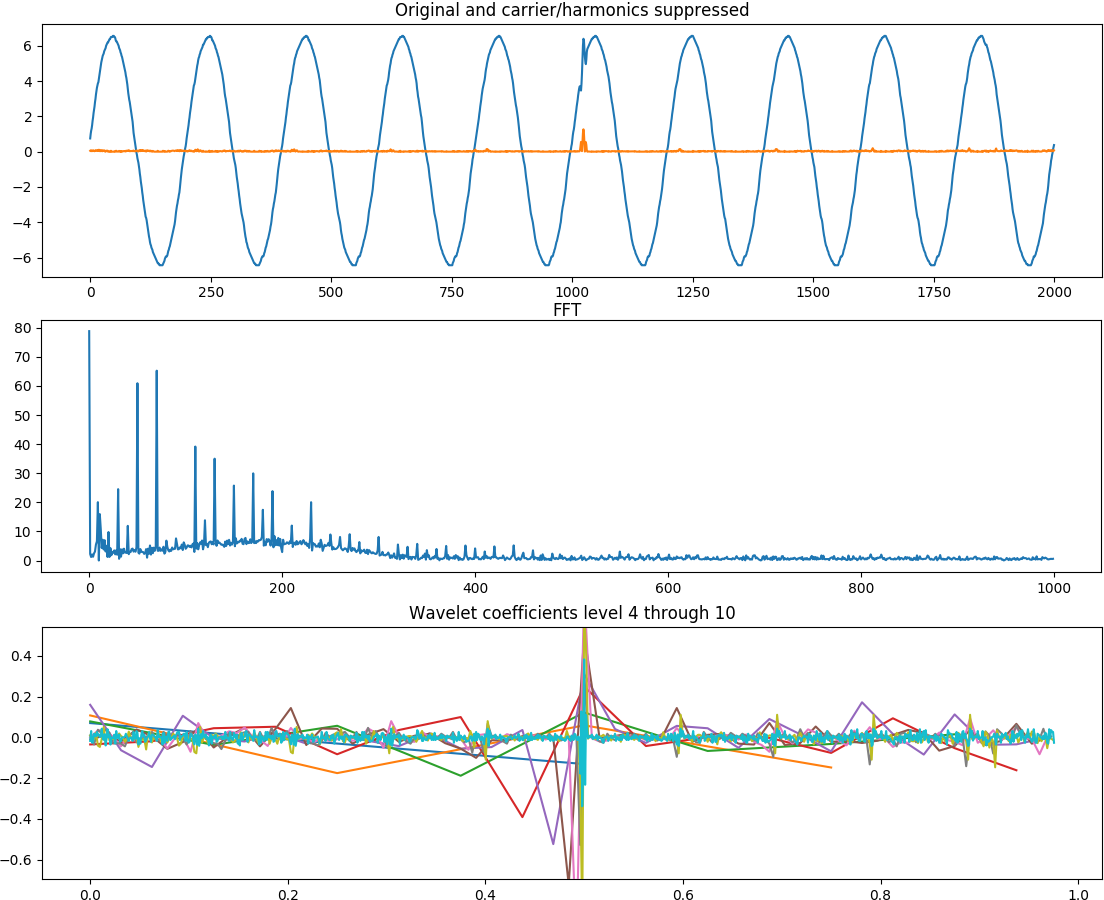
\includegraphics[width=0.8\linewidth]{img/proposed_detection.png}	
	\caption{Steps of the wavelet anomaly detection metric algorithm. Top: simulated transient superimposed with filtered version. Middle: FFT of the filtered data. Bottom: Discrete wavelet transform of filtered data.}
	\label{expdes:fig:1}
\end{figure}

It should be noted that the wavelet anomaly detection metric is sensitive to voltage sags and swells, and frequency deviations. The FFT base filtering step will leave a significant residual in both of these cases, and the wavelet coefficients will grow quite large as shown in figure \ref{expdes:fig:2}. However in these cases the temporal position and level of the highest coefficient does not provide a good localization of the disturbance. Wavelet anomaly detection metric was the only metric used in the triggering stream, it would be nearly impossible to perform temporal intra-window localization between multiple devices. On the other hand, windowed frequency and $V_{rms}$ metrics are quite capable of detecting this type of disturbance. Wavelet anomaly detection metric is completely insensitive to THD changes, since the the first step involves filtering the mains frequency and its harmonics. Unlike the three existing metrics, wavelet anomaly detection metric is sensitive to sudden, asynchronous changes in the input, and detection efficiency does not depend on length of the processing window. This compliments THD, $v_{rms}$ and frequency metrics, which are better suited for monitoring long term (1 cycle or more) changes.

\begin{figure}[h]
	\centering
	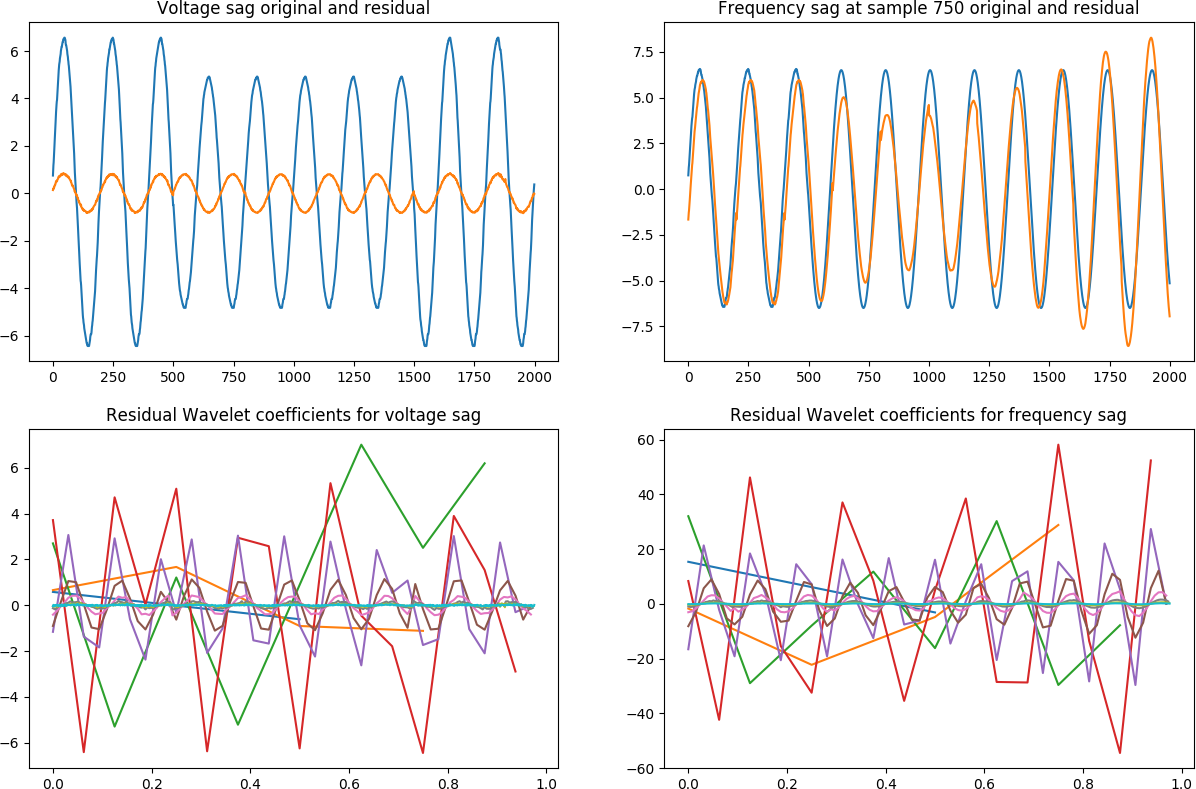
\includegraphics[width=0.8\linewidth]{img/sag_and_freq_wavelet.png}	
	\caption{Wavelet anomaly detection metric algorithm applied to a voltage sag(Left), and a 1\% frequency sag(Right)}.
	\label{expdes:fig:2}
\end{figure}

Once wavelet anomaly detection metric is integrated into the triggering stream, OPQMakai will be modified to use it for anomaly detection. OPQMakai will be able to dynamicaly vary the length of the processed window, decreasing it if a possible anomaly is taking place, and relaxing it once steady state is achieved. Furthermore since the location of the possible anomaly in the triggering window is provided by the anomaly metric, temporal correlation between multiple OPQBox devices will remain accurate even with relatively long triggering window. Frequency and $V_{rms}$ metrics will supersede the wavelet anomaly detection metric, since it is sensitive but ambiguous for the type of disturbances they are meant to detect. However if the frequency and $V_{rms}$ metrics are nominal, and the wavelet anomaly detection metric shows a disturbance, the triggering system will interpret this condition as a possible transient.

In order to validate the detection capabilities of the OPQBox it will be subjected to a set of synthetic benchmarks. A waveform generator will be employed to generate various PQ desturbances, which will be fed into the OPQBox. The resulting metrics will be analyzed to fine-tune the triggering thresholds and pattern matching, and the results will be compared to the industries standards. This work is expected to be carried out from September to October of 2018, and should result in a small instrumentation publication describing the detection capabilities of the OPQBox2.

In order to validate OPQ system as a whole it will be deployed across the University of Hawaii Manoa campus(UH). This location is ideal because it is a relatively isolated microgrid connected to the Oahu powergrid only via a single 46kV feeder as shown in figure \ref{expdes:fig:1}. Another advantage of the UH campus is the high number of smart meters deployed, across various levels of the power delivery infrastructure. While these meters are mainly geared towards monitoring power consumption they do have some power quality monitoring capabilities. Data provided from these meters can be used in two distinct applications. First of all, this data can be used to pinpoint the section of the University of Hawaii power grid which experience a higher likelihood of power quality disturbances. These portions of the grid will have a higher spacial density of OPQBoxes. Secondly, data from the campus deployed meters can be used as ground truth for comparison against the measurements, and analysis performed by the OPQ project. The location of smart meters in the grid topology is shown in figure \ref{expdes:fig:1} as the $M$ nodes. As evident by the meter location none of them are monitoring the consumer level power and mainly focus on the higher voltage power delivery. This placement is evidenced from the smart meter role as a consumption monitor, and thus the deployment of the OPQBoxes at the residential level will compliment the current power quality monitoring capabilities without introducing redundancies. Finally University of Hawaii powergrid is supplying a highly diverse infrastructure. Beyond the traditional residential equipment such as computers and consumer grade electronics, UH power grid powers scientific and laboratory equipment, machine shops, and server farms. All of these elements have varying requirements/tolerances for power quality anomalies as well as different levels of power quality "pollution". Furthermore some of the electricity consumers in the UH campus is entirely unique. For example the free electron laser located in the Watanabe Hall is one of the only free electron lasers in the world, and the impact/sensitivity of power quality on the instrument are completely unstudied.
\begin{figure}[h]
	\centering
	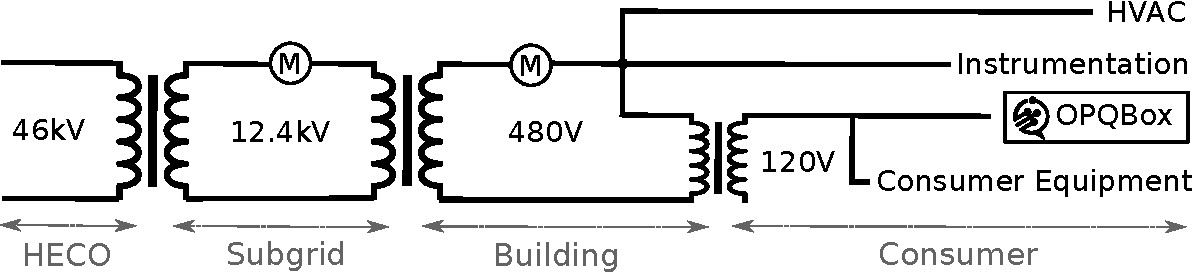
\includegraphics[width=1\linewidth]{img/uh-grid.pdf}	
	\caption{University of Hawaii at Manoa power delivery infrastructure.}
	\label{expdes:fig:3}
\end{figure}

Open power quality project acquired cloud infrastructure from the the Information Technology Services of University of Hawaii, which is hosted on the Manoa campus. This allows for low latency operation, and keeps all of the traffic constrained to the UH internal network. Furthermore UH hosts a Stratum 1 NTP server on its campus. This provides UH OPQ deployment with a low latency, high precision time keeping option. Finally, OPQ project received the Presidents Green Initiative Award in spring 2018. Besides a \$10,000 monetary award, this provides the OPQ project with access to all of the buildings on campus, expertise of the engineers who oversee the campus power infrastructure, as well as access to all of the smart meter measurements already deployed across campus. 

There are 74 smart meters deployed across the UH campus. These meters measure $V_{rms}$, power consumption, reactive power, and power factor. Power factor and reactive power are measurements of the ratio of useful power delivery to the total power delivery. With the power factor of 1, all of the power delivered to the load is used, with the power factor of 0.5 only half of the power can be used to do useful work, power factor of 0 means that all of the power delivered is wasted. Power factor, is a non-linear combinations of two metrics:
\begin{itemize}
  \item \textbf{Displacement power factor}: Phase lag between the current and voltage waveform. Since the power consumption is a product of current and voltage, $180^{\circ}$ phase difference between the two would result in power factor of 0.
  \item \textbf{Total harmonic distortion}: Non-linear loads only consume power during a short part of the AC cycle. This non-linear current waveform introduces harmonics into the current and voltage waveform, which impacts the power factor.
\end{itemize}
OPQBox is not capable of measuring displacement power factor, or the current total harmonic distortion directly. However since the output impedance of the power grid is non-zero, the current harmonic distortion will result in the voltage harmonic distortion, which OPQBox is quite capable of measuring. Since the smart meters are already measuring power factor, combining their measurements with the THD measured by the OPQbox, will allow UH engineers to attribute low power factor measurements to one of the two underlying causes. Since the solution to the displacement power factor and THD issues are entirely different, this will streamline the debugging of the power factor issues.

OPQBoxes measure $V_{rms}$ as part of their triggering stream. As shown in equation \ref{eq:3} OPQBox computes the the $V_{rms}$ value by combining the values of ten cycles. With the sampling rate of 12kSps, each $V_{rms}$ measurement of the OPQBox is a result of processing 2000 samples. The smart meters deployed across campus, sample at 1kHz, and thus may miss shortlived power quality events to aliasing. Furthermore the readings from the smart meters are reported at 2 second intervals an thus, short lived sags and swells will be averaged out from the reported data. OPQBoxes however will be able to detect most of the $V_{rms}$ disturbances detected by the UH smartmeeters, since sags and swells, tend to propagate down the power distribution hierarchy and the OPQBoxes make up the leafs of the monitoring infrastructure, and offer supperior $V_{rms}$ detection capabilities.

OPQBoxes report the fundamental frequency as part of their triggering stream. The fundamental frequency is averaged across a window of 10 grid cycles, and sent to the OpqHub 6 times a second, however as the system evolves the window width will be adjustable. In synthetic benchmarks OPQBox2 outperforms the stated precision of the UHM meters, and as such OPQBox2 measurements can be directly compared to the installed meters.

Transient detection is not implemented on the on the UHM meters, and as such there is no direct comparison for detection efficiency across the two systems. However the UHM meters provide an API for receiving live data. It should be possible to implement a system where the live raw data from the smart meters is requested for triggered events. This will provide a full picture of the transient propagation across the UH power grid, string form the 48kV feeder, down the the consumer outlet.

OPQ system will make a valuable addition to the power grid infrastructure at the University of Hawaii. It will provide UHM engineers with a tool for debugging power quality issues at the consumer level across the entire branch of the power delivery system. Furthermore it will provide a testbed for developing PQ anomaly detection without having to development of addition monitoring infrastructure. Finally, the detected event database will provide a good dataset for PQ classification and disturbance propagation analysis.

Data collected via the OPQ deployment at the UHM campus will be unique, since it will combine waveforms from both the edge and the distribution level meters. This data will allow me to validate the hypothesis that monitoring power infrastructure at the leaf edges is sufficient to determine where in the hierarchical power grid system the PQ disturbances originated. Currently the OPQBox2 is being redesigned to be suitable for mass production. This redesign includes a new single sided PCB to reduce assembly cost, a new off-the-shelf enclosure which saves assembly time, as well as a new software stack which makes it easier to add and modify the OPQBox analysis stack. Once the new OPQBox is ready to deployment up to 100 devices will be deployed across the UH campus(the exact number depends on the final per unit cost). I expect to have a full deployment in late October to facilitate a two month data collection period. 

Once the data is collected, the rigorous analysis of comparing the results from the UHM meters and the OPQ system will begin. The goal of this analysis is to demonstrate the capabilities of the OPQ system to monitor and localize PQ anomalies by only monitoring the edge of the power distribution infrastructure. I expect the analysis to take start in January 2019 and finish at the end of February of 2019. The resulted analysis will form a core of a OPQ system publication which will be published in Summer of 2019. The full schedule of proposed activities is shown below:

\begin{center}
\begin{tabular}{ ||c | c c|| }
\hline
 \textbf{Activity} & \textbf{Start Date} & \textbf{End Date} \\ 
 \hline
 \hline
 OPQBox2 Validation & September 1\textsuperscript{st} & October 31\textsuperscript{st} \\  
 OPQBox2 Deployment & November 1\textsuperscript{st} & November 30\textsuperscript{th}   \\
 Data Collection & December 1\textsuperscript{st} & February 1\textsuperscript{st}   \\
 OPQBox2 Instrumentation paper & January 1\textsuperscript{st} & February 1\textsuperscript{st}   \\
 Data Analysis & February 1\textsuperscript{st} & March 1\textsuperscript{st}  \\
 \hline
 
\end{tabular}
\end{center}
